
\subsection*{Mathematical Derivation of the VAM-Lagrangian}

Kinetic energy of a vortex structure, or the local energy density in a vortex field:

\[
\mathcal{L}_\text{kin} = \frac{1}{2}\rho_\text{\ae} C_e^2
\]

Veddy field energy and gauge terms, field tensors follow from Helmholtz vorticity:

\[
\mathcal{L}_\text{veld} = -\frac{1}{4}F_{\mu\nu}F^{\mu\nu}
\]

Veddy mass as inertia from circulation, where the fermion mass is determined by circulation:
\[
\Gamma = 2\pi r_c C_e \quad\Rightarrow\quad m \sim \rho_\text{\ae} r_c^3
\]

Pressure and stress potential of æther condensate, where the pressure balance is described by the stress field:
\[
V(\phi) = -\frac{F_\text{max}}{r_c}|\phi|^2 + \lambda|\phi|^4
\]

Topological terms for the conservation of vortex fields helicity:
\[
\mathcal{H} = \int \vec{v}\cdot\vec{\omega}\, dV
\]

\subsection*{Supporting Experimental and Theoretical Observations}
The VAM is consistent with experimentally and theoretically confirmed phenomena such as vortex stretching, helicity conservation and mass-inertia couplings \cite{batchelor1953,vinen2002,bewley2008,moffatt1969,kleckner2013,scheeler2014,bartlett1986}.


\section{Topological Origins of Particle Properties in VAM}

In the Vortex Æther Model (VAM), fundamental particles are not point-like but correspond to stable, quantized vortex knots within a compressible, rotating æther medium. Each property typically assigned by quantum field theory---mass, charge, spin, and flavor---is instead interpreted as a manifestation of topological and dynamical characteristics of the underlying vortex structure.

\subsection{Mass as a Function of Circulation and Core Geometry}

Particle mass in VAM is not fundamental but derived from the energy stored in vortex tension and helicity. For a single knot with circulation $\Gamma$, core radius $r_c$, and æther density $\rho_{\text{\ae}}$, the mass is:

\begin{equation}
m_f = \frac{\rho_{\text{\ae}} \Gamma^2}{3\pi r_c C_e^2}
\end{equation}

\begin{figure}[h!]
\centering
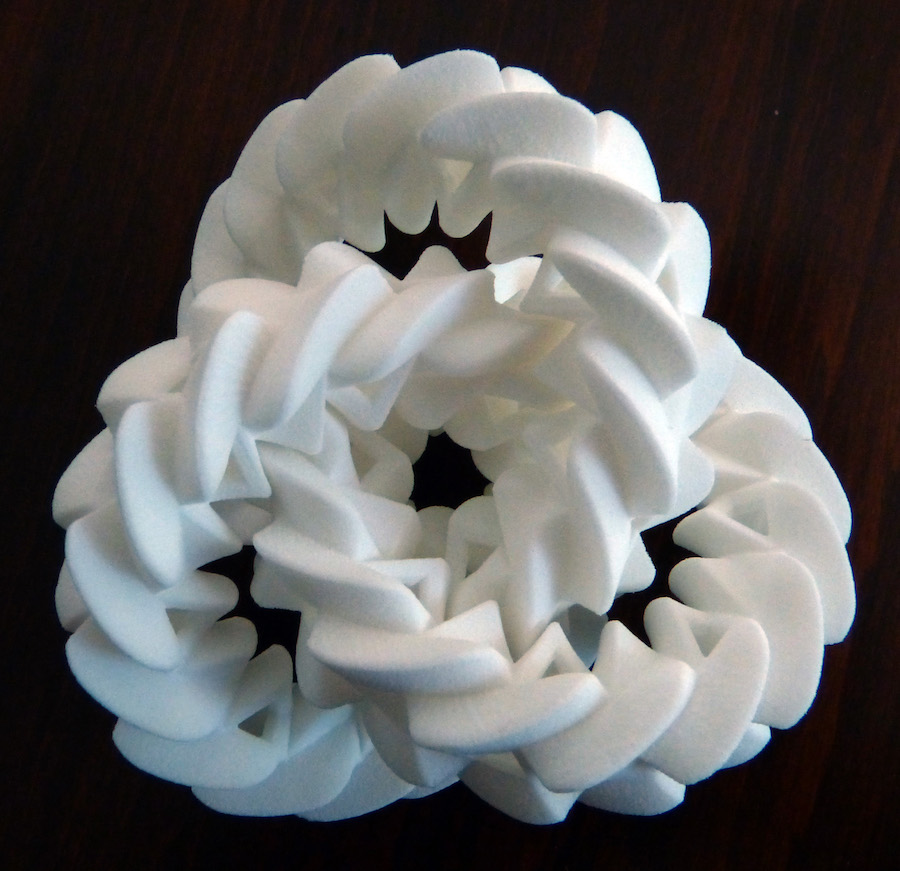
\includegraphics[width=0.65\textwidth]{mechanic trefoil}
\caption{Mechanical model of coupled nodal vertebra, visually analogous to inertia.}
\end{figure}

This quantity scales with the square of circulation, inversely with core size, and depends directly on the background æther density. Mass hierarchies between generations may result from different topological classes (e.g., torus knots vs. prime knots) and chirality.

\subsection{Spin from Quantized Vortex Angular Momentum}

Spin-$\tfrac{1}{2}$ particles are modeled as topological solitons with intrinsic angular momentum arising from locked circulation patterns. Each fermionic knot carries quantized angular momentum:

\begin{equation}
S = \frac{1}{2} \hbar_\text{VAM} = \frac{1}{2} m_f C_e r_c
\end{equation}

This links the classical notion of rotation directly to quantum spin and validates the half-integer nature as a result of geometric twist.

\subsection{Charge via Swirl Chirality and Helicity Direction}

Electric charge is modeled as a geometric property of the swirl’s handedness and linkage to background vorticity. Positive and negative charges correspond to opposite helicity configurations, with magnitude determined by:

\begin{equation}
q \propto \oint \vec{v} \cdot d\vec{l} = \Gamma
\end{equation}

The fine-structure constant $\alpha$ arises from the dimensionless ratio:

\begin{equation}
\alpha = \frac{q^2}{4\pi \epsilon_0 \hbar c} \quad \Rightarrow \quad \alpha = \frac{2C_e}{c}
\end{equation}

This shows that $\alpha$ is no longer a free parameter but a function of swirl velocity in the æther relative to light speed.

\subsection{Flavor and Generation from Topological Class}

Higher-generation particles are interpreted as more complex knots---e.g., double torus knots, linked loops, or braid configurations---with each class inducing distinct stability conditions and oscillation modes. Lepton and quark families thus correspond to increasing knot complexity, not arbitrary quantum numbers.

\subsection{Color and Confinement via Vortex Bundle Interactions}

Color charge and confinement emerge from multi-vortex bundles, where topological stability requires trivalent junctions (akin to QCD gluon vertices). Individual color states are unstable in isolation due to their open helicity paths and unbalanced tension.

\bigskip

This mapping from abstract quantum numbers to geometric vortex properties transforms the ontology of matter: particles are not elementary but emergent solitonic knots, with observable traits arising from fluidic topology, circulation, and helicity alignment within the æther medium.
